\section{Burgers' equation: an exactly solvable model}

The one dimensional Burgers equation
\[
\partial_tu+u\,\partial_xu = \nu\,\partial_x^2u
\]
shares the quadratic nonlinearity and the dissipation of Navier Stokes but none of its geometric complexity, and it can be solved exactly. Hopf~\cite{hopf1950} and Cole~\cite{cole1951} observed in 1950 and 1951 that the substitution $u = -2\nu\,\partial_x\log\phi$ transforms it into the heat equation $\partial_t\phi = \nu\,\partial_x^2\phi$. With $u_0 = U_0'$, the solution is
\[
u(t,x) = \frac{\int\frac{x-y}{t}\exp\big(-\frac{(x-y)^2}{4\nu t}-\frac{U_0(y)}{2\nu}\big)\dd y}{\int\exp\big(-\frac{(x-y)^2}{4\nu t}-\frac{U_0(y)}{2\nu}\big)\dd y}.
\]
The formula has a Bayesian reading that is exact. Regard $y$ as an unknown initial position, give it the improper prior proportional to $e^{-U_0(y)/2\nu}$, and observe the position $x$ of a Brownian particle with diffusion coefficient $\nu$ at time $t$. Then $u(t,x) = \E[(x-Y)/t\mid x]$, the posterior mean of the average velocity of the particle given its endpoint. The Hopf Cole transform is the Feynman Kac formula of Chapter~\ref{ch:quantum} for the heat equation.

As $\nu\to0$, Laplace's method replaces the posterior mean by the posterior mode, the minimizer of $\frac{(x-y)^2}{2t}+U_0(y)$, which is the Hopf Lax formula of the inviscid equation. Where the minimizer jumps, the solution has a shock. Figure~\ref{fig:burgers} shows the solution for three viscosities: as $\nu$ decreases, the profile steepens into a shock. The energy dissipation rate $\nu\int(\partial_xu)^2\dd x$ does not vanish as $\nu\to0$ once a shock forms: the gradient grows like $1/\nu$ over a layer of width $\nu$, so the dissipation converges to a positive limit determined by the jump. This is anomalous dissipation in its simplest form, the one dimensional caricature of Onsager's mechanism, and it is rigorous. In the posterior language, a shock is a point at which the posterior over initial positions becomes bimodal: two different initial points are equally good explanations of the observed position, and the limit selects between them discontinuously.

\begin{figure}[t]
\centering
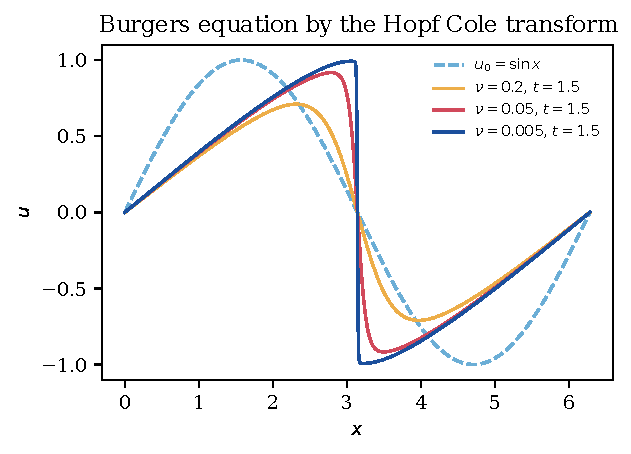
\includegraphics[width=0.92\textwidth]{burgers}
\caption{Solutions of the Burgers equation at $t=1.5$ for $\nu=0.2$, $0.05$ and $0.005$, computed by quadrature of the Hopf Cole formula from the initial condition $u_0=\sin x$, which is also drawn. The shock at $x=\pi$ forms in the inviscid limit.}
\label{fig:burgers}
\end{figure}

Burgers turbulence, the statistical theory of Burgers equation with random initial data or forcing, was developed by Sinai~\cite{sinai1992}, by E, Khanin, Mazel and Sinai~\cite{ekms2000}, and by others. For forcing that is periodic in space and white in time the inviscid equation has a unique invariant measure~\cite{ekms2000}, described through one sided minimizers of the action, and the structure functions scale as $S_p(\ell)\propto\ell$ for $p\geq1$ as $\ell\to0$~\cite{evandeneijnden2000}, a pure bifractal intermittency caused by the shocks. The exponents are therefore known exactly, which makes the model a test case for statistical methods that estimate scaling exponents from data.

\section{Inferring the dissipation rate}\label{sec:infer_dissipation}

The four fifths law gives a moment equation for $\varepsilon$, but in practice the inertial range is short and the third order structure function is noisy. A Bayesian model combines all scales. Let $\delta u_\parallel(\ell_j)$ be measured longitudinal increments at separations $\ell_1<\dots<\ell_J$. Conditionally on a local dissipation $\varepsilon_\ell$ at scale $\ell$, the K62 hypothesis gives increments of the form $\delta u\approx(\varepsilon_\ell\ell)^{1/3}Z$ with $Z$ a skewed variable independent of $\varepsilon_\ell$ and $\E Z^3 = -\frac45$, and $\log\varepsilon_\ell$ Gaussian with mean $\log\varepsilon-\frac{\mu}{2}\log(L/\ell)$ and variance $\mu\log(L/\ell)$, where $\mu$ is the intermittency coefficient. The mean and variance give $\E\varepsilon_\ell = \varepsilon$, so that $\E(\delta u)^3 = \ell\,\E\varepsilon_\ell\,\E Z^3 = -\frac45\varepsilon\ell$, which is the four fifths law. The model is a scale mixture in the sense of Chapter~\ref{ch:mixtures}, with lognormal mixing, and data augmentation over the latent $\varepsilon_\ell$ gives a posterior for $(\varepsilon,\mu,L)$ that can be sampled by Markov chain Monte Carlo. For a general law of $Z$ the lognormal mixing is not conjugate and the sampler needs Metropolis steps. We have not carried out the computation. The posterior of $\mu$ would be the statistical quantity behind the debate over the departure of structure function exponents from $p/3$, and the posterior of $\varepsilon$ given finite resolution data would quantify how sharply the anomalous dissipation hypothesis can be tested.

\section*{Exercises}
\begin{enumerate}
\item Verify that the Hopf Cole substitution transforms the Burgers equation into the heat equation.
\item Write the stationary elliptic system satisfied by a Leray self similar profile $U$.
\item Derive Fieller's interval for the ratio of two jointly Gaussian quantities with known covariance.
\item Using the scaling $u_\lambda(t,x) = \lambda^{2\alpha-1}u(\lambda^{2\alpha}t,\lambda x)$, show that the energy is critical for the hypodissipative equations in three dimensions exactly when $\alpha = 5/4$.
\item For the inviscid Burgers equation with $u_0 = \sin x$, show that the shock forms at time one.
\end{enumerate}
